\documentclass[]{beamer}\usepackage[]{graphicx}\usepackage[]{color}
% maxwidth is the original width if it is less than linewidth
% otherwise use linewidth (to make sure the graphics do not exceed the margin)
\makeatletter
\def\maxwidth{ %
  \ifdim\Gin@nat@width>\linewidth
    \linewidth
  \else
    \Gin@nat@width
  \fi
}
\makeatother

\definecolor{fgcolor}{rgb}{0.345, 0.345, 0.345}
\newcommand{\hlnum}[1]{\textcolor[rgb]{0.686,0.059,0.569}{#1}}%
\newcommand{\hlstr}[1]{\textcolor[rgb]{0.192,0.494,0.8}{#1}}%
\newcommand{\hlcom}[1]{\textcolor[rgb]{0.678,0.584,0.686}{\textit{#1}}}%
\newcommand{\hlopt}[1]{\textcolor[rgb]{0,0,0}{#1}}%
\newcommand{\hlstd}[1]{\textcolor[rgb]{0.345,0.345,0.345}{#1}}%
\newcommand{\hlkwa}[1]{\textcolor[rgb]{0.161,0.373,0.58}{\textbf{#1}}}%
\newcommand{\hlkwb}[1]{\textcolor[rgb]{0.69,0.353,0.396}{#1}}%
\newcommand{\hlkwc}[1]{\textcolor[rgb]{0.333,0.667,0.333}{#1}}%
\newcommand{\hlkwd}[1]{\textcolor[rgb]{0.737,0.353,0.396}{\textbf{#1}}}%
\let\hlipl\hlkwb

\usepackage{framed}
\makeatletter
\newenvironment{kframe}{%
 \def\at@end@of@kframe{}%
 \ifinner\ifhmode%
  \def\at@end@of@kframe{\end{minipage}}%
  \begin{minipage}{\columnwidth}%
 \fi\fi%
 \def\FrameCommand##1{\hskip\@totalleftmargin \hskip-\fboxsep
 \colorbox{shadecolor}{##1}\hskip-\fboxsep
     % There is no \\@totalrightmargin, so:
     \hskip-\linewidth \hskip-\@totalleftmargin \hskip\columnwidth}%
 \MakeFramed {\advance\hsize-\width
   \@totalleftmargin\z@ \linewidth\hsize
   \@setminipage}}%
 {\par\unskip\endMakeFramed%
 \at@end@of@kframe}
\makeatother

\definecolor{shadecolor}{rgb}{.97, .97, .97}
\definecolor{messagecolor}{rgb}{0, 0, 0}
\definecolor{warningcolor}{rgb}{1, 0, 1}
\definecolor{errorcolor}{rgb}{1, 0, 0}
\newenvironment{knitrout}{}{} % an empty environment to be redefined in TeX

\usepackage{alltt}
%\documentclass[handout]{beamer}

\usepackage{graphicx}
\usepackage{amsmath,amssymb,array,comment,eucal}
\usepackage{xcolor}
\definecolor{beamer@blendedblue}{RGB}{86,155,189}
\definecolor{myblue}{RGB}{12,76,138}
\setbeamercolor{structure}{fg=myblue}
\definecolor{Ftitle}{RGB}{12,76,138}
\definecolor{Descitem}{RGB}{238,238,244}
\definecolor{StdTitle}{RGB}{12,76,138}
\definecolor{StdBody}{RGB}{213,24,0}
\definecolor{StdBody}{RGB}{213,24,0}

\definecolor{AlTitle}{RGB}{255, 190, 190}
\definecolor{AlBody}{RGB}{213,24,0}

\definecolor{ExTitle}{RGB}{201, 217, 217}
\definecolor{ExBody}{RGB}{213,24,0}

\setbeamercolor{frametitle}{fg = Ftitle}
\setbeamercolor{title}{fg = Ftitle}
\setbeamercolor{item}{fg = Ftitle}
\setbeamercolor{subitem}{fg = Ftitle}
\setbeamercolor{subsubitem}{fg = Ftitle}
\setbeamercolor{description item}{fg = myblue}
\setbeamercolor{titlelike}{fg=myblue}

\DeclareMathOperator{\sgn}{sgn}
\newcommand{\e}{\mathbf{e}}
\renewcommand{\P}{\mathbf{P}}
\newcommand{\F}{\mathbf{F}}
\newcommand{\R}{\textsf{R}}
\newcommand{\mat}[1] {\mathbf{#1}}
%\newcommand{\ind}{\mathrel{\mathop{\sim}\limits^{\mathit{ind}}}}
%\newcommand{\iid}{\mathrel{\mathop{\sim}\limits^{\mathit{iid}}}}
\newcommand{\E}{\textsf{E}}
\newcommand{\SE}{\textsf{SE}}
\newcommand{\SSE}{\textsf{SSE}}
\newcommand{\RSS}{\textsf{RSS}}
\newcommand{\FSS}{\textsf{FSS}}
\renewcommand{\SS}{\textsf{SS}}
\newcommand{\MSE}{\textsf{MSE}}
\newcommand{\SSR}{\textsf{SSR}}
\newcommand{\Be}{\textsf{Beta}}
\newcommand{\St}{\textsf{St}}
\newcommand{\Ca}{\textsf{C}}
\newcommand{\Exp}{\textsf{Exp}}
\newcommand{\GDP}{\textsf{GDP}}
\newcommand{\NcSt}{\textsf{NcSt}}
\newcommand{\Bin}{\textsf{Bin}}
\newcommand{\NB}{\textsf{NegBin}}
\renewcommand{\NG}{\textsf{NG}}
\newcommand{\N}{\textsf{N}}
\newcommand{\Ber}{\textsf{Ber}}
\newcommand{\Poi}{\text{Poi}}
\newcommand{\Gam}{\textsf{Gamma}}
\newcommand{\BB}{\textsf{BB}}
\newcommand{\Gm}{\textsf{G}}
\newcommand{\Un}{\textsf{Unif}}
\newcommand{\Ex}{\textsf{Exp}}
\newcommand{\DE}{\textsf{DE}}
\newcommand{\tr}{\textsf{tr}}
\newcommand{\cF}{{\cal{F}}}
\newcommand{\cL}{{\cal{L}}}
\newcommand{\cI}{{\cal{I}}}
\newcommand{\cB}{{\cal{B}}}
\newcommand{\cP}{{\cal{P}}}
\newcommand{\bbR}{\mathbb{R}}
\newcommand{\bbN}{\mathbb{N}}
\newcommand{\pperp}{\mathrel{{\rlap{$\,\perp$}\perp\,\,}}}
\newcommand{\OFP}{(\Omega,\cF, \P)}
\newcommand{\eps}{\boldsymbol{\epsilon}}
\newcommand{\1}{\mathbf{1}_n}
\newcommand{\gap}{\vspace{8mm}}
\newcommand{\ind}{\mathrel{\mathop{\sim}\limits^{\rm ind}}}
\newcommand{\simiid}{\ensuremath{\mathrel{\mathop{\sim}\limits^{\rm
iid}}}}
\newcommand{\eqindis}{\ensuremath{\mathrel{\mathop{=}\limits^{\rm D}}}}
\newcommand{\iid}{\textit{i.i.d.}}
\newcommand{\SSZ}{S_{zz}}
\newcommand{\SZW}{S_{zw}}
\newcommand{\Var}{\textsf{Var}}
\newcommand{\corr}{\textsf{corr}}
\newcommand{\diag}{\textsf{diag}}
\newcommand{\var}{\textsf{var}}
\newcommand{\Cov}{\textsf{Cov}}
\newcommand{\Sam}{{\cal S}}
\def\H{\mathbf{H}}
\newcommand{\I}{\mathbf{I}}
\newcommand{\Y}{\mathbf{Y}}
\newcommand{\tY}{\tilde{\mathbf{Y}}}
\newcommand{\Yhat}{\hat{\mathbf{Y}}}
\newcommand{\Yobs}{\mathbf{Y}_{{\cal S}}}
\newcommand{\barYobs}{\bar{Y}_{{\cal S}}}
\newcommand{\barYmiss}{\bar{Y}_{{\cal S}^c}}
\def\bv{\mathbf{b}}
\def\X{\mathbf{X}}
\def\tX{\tilde{\mathbf{X}}}
\def\x{\mathbf{x}}
\def\xbar{\bar{\mathbf{x}}}
\def\Xbar{\bar{\mathbf{X}}}
\def\Xg{\mathbf{X}_{\boldsymbol{\gamma}}}
\def\Ybar{\bar{\Y}}
\def\ybar{\bar{y}}
\def\y{\mathbf{y}}
\def\Yf{\mathbf{Y_f}}
\def\W{\mathbf{W}}
\def\L{\mathbf{L}}
\def\w{\mathbf{w}}
\def\U{\mathbf{U}}
\def\V{\mathbf{V}}
\def\Q{\mathbf{Q}}
\def\Z{\mathbf{Z}}
\def\z{\mathbf{z}}
\def\v{\mathbf{v}}
\def\u{\mathbf{u}}

\def\zero{\mathbf{0}}
\def\one{\mathbf{1}}
\newcommand{\taub}{\boldsymbol{\tau}}
\newcommand{\betav}{\boldsymbol{\beta}}
\newcommand{\alphav}{\boldsymbol{\alpha}}
\newcommand{\A}{\mathbf{A}}
\def\a{\mathbf{a}}
\def\K{\mathbf{K}}
\newcommand{\B}{\mathbf{B}}
\def\b{\boldsymbol{\beta}}
\def\bhat{\hat{\boldsymbol{\beta}}}
\def\btilde{\tilde{\boldsymbol{\beta}}}
\def\tb{\boldsymbol{\theta}}
\def\bg{\boldsymbol{\beta_\gamma}}
\def\bgnot{\boldsymbol{\beta_{(-\gamma)}}}
\def\mub{\boldsymbol{\mu}}
\def\tmub{\tilde{\boldsymbol{\mu}}}
\def\muhat{\hat{\boldsymbol{\mu}}}
\def\tb{\boldsymbol{\theta}}
\def\tk{\boldsymbol{\theta}_k}
\def\tj{\boldsymbol{\theta}_j}
\def\Mk{\boldsymbol{{\cal M}}_k}
\def\M{\boldsymbol{{\cal M}}}
\def\Mj{\boldsymbol{{\cal M}}_j}
\def\Mi{\boldsymbol{{\cal M}}_i}
\def\Mg{{\boldsymbol{{\cal M}_\gamma}}}
\def\Mnull{\boldsymbol{{\cal M}}_{N}}
\def\gMPM{\boldsymbol{\gamma}_{\text{MPM}}}
\def\gHPM{\boldsymbol{\gamma}_{\text{HPM}}}
\def\Mfull{\boldsymbol{{\cal M}}_{F}}
\def\tg{\boldsymbol{\theta}_{\boldsymbol{\gamma}}}
\def\g{\boldsymbol{\gamma}}
\def\eg{\boldsymbol{\eta}_{\boldsymbol{\gamma}}}
\def\G{\mathbf{G}}
\def\cM{\cal M}
\def\D{\Delta}
\def \shat{{\hat{\sigma}}^2}
\def\uv{\mathbf{u}}
\def\l {\lambda}
\def\d{\delta}
\def\Sigmab{\boldsymbol{\Sigma}}
\def\Lambdab{\boldsymbol{\Lambda}}
\def\lambdab{\boldsymbol{\lambda}}
\def\Mg{{\cal M}_\gamma}
\def\S{{\cal{S}}}
\def\qg{p_{\boldsymbol{\gamma}}}
\def\pg{p_{\boldsymbol{\gamma}}}
%\def\t{\mathbf{t}}
\def\T{\boldsymbol{\Theta}}
\def\Tb{\boldsymbol{\Theta}}
\def\t{\mathbf{t}}

\usepackage{verbatim}

\usetheme{default}
\title{Shrinkage Estimation \& Ridge Regression}
\subtitle{Readings Chapter 15 Christensen}
\institute{Merlise Clyde}
\author{STA721 Linear Models Duke University}
\date{\today}
\IfFileExists{upquote.sty}{\usepackage{upquote}}{}
\begin{document}
\maketitle

\begin{frame}
  \frametitle{How Good are Bayes Estimators?}
Quadratic loss for estimating  $\b$ using estimator $\a$
$$ L(\b, \a) =  ( \b - \a)^T(\b -\a)$$ \pause

\begin{itemize}
\item Consider our expected loss (before we see the data) of taking an
``action'' $\a$ (the estimate that we report)\pause
\item Under OLS or the  Reference prior the Expected Mean Square Error  \pause
  \begin{eqnarray*}
\E_\Y[( \b - \bhat)^T(\b -\bhat) & = &\sigma^2
  \tr[(\X^T\X)^{-1}] \pause \\
 & = & \sigma^2 \sum_{j=1}^p \lambda_j^{-1}
  \end{eqnarray*}
where $\lambda_j$ are eigenvalues of $\X^T\X$.
\pause
\item If smallest $\lambda_j \to 0$ then MSE  $\to \infty$
\item Note: estimate is unbiased!
\end{itemize}
\end{frame}

\begin{frame}
  \frametitle{Is the $g$-prior better?}

\begin{itemize}
  \item

\item Explore Frequentist properties of using a Bayesian estimator
$$\E_\Y[( \b - \bhat_g)^T(\b -\bhat_g)$$
but now $\bhat_g = g/(1+g) \bhat$  \pause

\item Sampling distribution of $\bhat_g  = \frac{g}{1+g}(\X^T\X)^{-1} \X^T\Y$  \pause
\item HW: show that there is a value of $g$ prior such that the g-prior is always better than the Reference prior/OLS

\item Potential problem: MSE also blows up if smallest eigenvalue goes to zero!
\end{itemize}
\end{frame}

\begin{frame}\frametitle{Estimator Properties}

  \begin{itemize}
  \item  Bias  \pause
  \item  Variance \pause
  \item MSE = Bias$^2$ + Variance  (multivariate analogs) \pause
\item Problems with OLS, g-priors \& mixtures of g-priors with collinearity \pause
\item Solutions: \pause
  \begin{itemize}
  \item removal of terms \pause
   \item other shrinkage estimators
  \end{itemize}

  \end{itemize}
\end{frame}






\begin{frame}
  \frametitle{Canonical Representation \& Ridge Regression}


  \begin{itemize}
\item  Assume that $\X$ has been centered and standardized so that $\X^T\X
  = \corr(\X)$ \pause  (use {\tt scale} or {\tt sweep} functions in {\tt R}) \pause
  \item Write $\X = \U_p L \V^T$ Singular Value Decomposition \pause where
    $\U_p^T\U_p = \I_p$ and $\V$ is $p \times p$ orthogonal matrix,
    $L$ is diagonal \pause
  $$ \Y = \one \alpha +  \U_p L \V^T \b + \eps $$ \pause
  \item  Let $\g =  \V^T \b$ and create
   $\U$   an $n \times n$  orthogonal matrix \pause
  $$\U = [\U_0 \, | \, \U_p \,| \,\U_{n-p-1}]$$
  where $\U_0 = \one/\sqrt{n}$  \pause
  \item $\U_0^T\U_p = 0$, $\U^T_0 \U_{n-p-1} = 0$ and  $\U_p^T\U_{n - p -1} = 0$ (orthogonal columns)
  \end{itemize}
\end{frame}
  \begin{frame} {Orthogonal Regression}
Rotate by multiplyting by $\U^T$:
  \begin{eqnarray*}
    \U^T \Y & = & \U^T \one \alpha + \U^T \U_p L \V^T \b + \U^T \eps \pause \\
    \Y^*
   &=& \left[
  \begin{array}{cc}
  \sqrt{n} & \zero_p^T\\ \zero_p & L \\  \zero_{n-p -1} & \zero_{n - p - 1  \times p}
  \end{array}
 \right]
\left(    \begin{array}{c}
      \alpha \\
  \g
    \end{array} \right)
+  \eps^*
  \end{eqnarray*} \pause


  \begin{itemize}
  \item   $y^*_0 \equiv \hat{\alpha} = \ybar$ \pause
\item $\hat{\g} =( L^TL)^{-1} L^T \U^T_p\Y$ or $\hat{\gamma}_i = y^*_i/l_i$ for
  $i = 1, \ldots, p$ \pause
\item  $\Var(\hat{\gamma}_i) = \sigma^2/l_i^2$
  \end{itemize}
Directions in $\X$ space $\U_j$ with small eigenvectors $l_i$ have
the largest variances.  Unstable directions.
\end{frame}

\begin{frame}
  \frametitle{Ridge  Regression \& Independent Prior}
  (Another) Normal Conjugate Prior Distribution on $\g$: $$\g \mid \phi \sim \N(\zero_p, \frac{1}{ \phi
    k} \I_p)$$ \pause

Posterior mean
$$
 \tilde{\g} =( L^TL + k \I)^{-1} L^T \U^T_p\Y  = ( L^TL + k \I)^{-1}
 L^TL\hat{\g}
$$\pause

 $$\tilde{\gamma}_i = \frac{l_i^2}{l_i^2 + k} \hat{\gamma}_i =
 \frac{\lambda_i}{\lambda_i + k} \hat{\gamma}_i $$ \pause
 \begin{itemize}
\item When $\lambda_i \to 0$ then $\tilde{\gamma}_i \to 0$

\item When $k \to 0$ we get OLS back but if $k$ gets too  big posterior
  mean goes to zero.
 \end{itemize}

\end{frame}
\begin{frame}
  \frametitle{Transform}
  \begin{itemize}
  \item
  Transform back $\tilde{\b} = \V \tilde{\g}$ \pause
  $$\tilde{\b} = (\X^T\X + k \I)^{-1}  \X^T\X \bhat$$ \pause
\item importance of standardizing \pause

\item Is there a value of $k$ for which ridge is better in terms of
  Expected MSE than OLS? \pause
\item Choice of $k$?
  \end{itemize}
\end{frame}
\begin{frame}\frametitle{MSE}
Can show that
 $$\E[(\b - \btilde)^T(\b - \btilde)] = \E[(\g - \tilde{\g})^T(\g - \tilde{\g}]$$
  \pause
 \begin{itemize}
 \item $\Var(\tilde{\gamma}_i) = \sigma^2 l_i^2 /(l_i^2 +
   k)^2$ \pause
\item  Bias of $\tilde{\g}$ is $-k \gamma_i/(l_i^2 + k)$ \pause
 \item  MSE $$\sigma^2 \sum_i \frac{l_i^2}{(l_i^2 + k)^2} +  k^2
   \sum_i \frac{\gamma_i^2} {(l_i^2 + k)^2} $$
 \end{itemize}
The derivative with respect to $k$ is negative at $k=0$, hence the
function is decreasing. \pause

\vspace{12pt}
Since $k = 0$ is OLS, this means that is a value of $k$ that will
always be better than OLS
\end{frame}

\begin{frame}  \frametitle{Alternative Motivation}
  \begin{itemize}
  \item If  $\bhat$ is unconstrained  expect high variance with nearly
    singular $\X$ \pause
  \item Let $\Y^c = (\I - \P_1) \Y$  and $\X^c$ the centered and
    standardized  $\X$ matrix \pause
\item Control how large coefficients may grow \pause
    $$\min_{\b} (\Y^c - \X^c \b)^T (\Y^c - \X^c\b)$$
    subject to
    $$ \sum \beta_j^2 \le t$$ \pause
  \item Equivalent Quadratic Programming Problem
    $$\min_{\b} \| \Y^c - \X^c \b\|^2 + k \|\b\|^2$$ \pause
  \item ``penalized'' likelihood \pause
  \end{itemize}
\end{frame}
\begin{frame}\frametitle{Picture}

\end{frame}
\begin{frame}
  \frametitle{Longley Data}
  \centerline{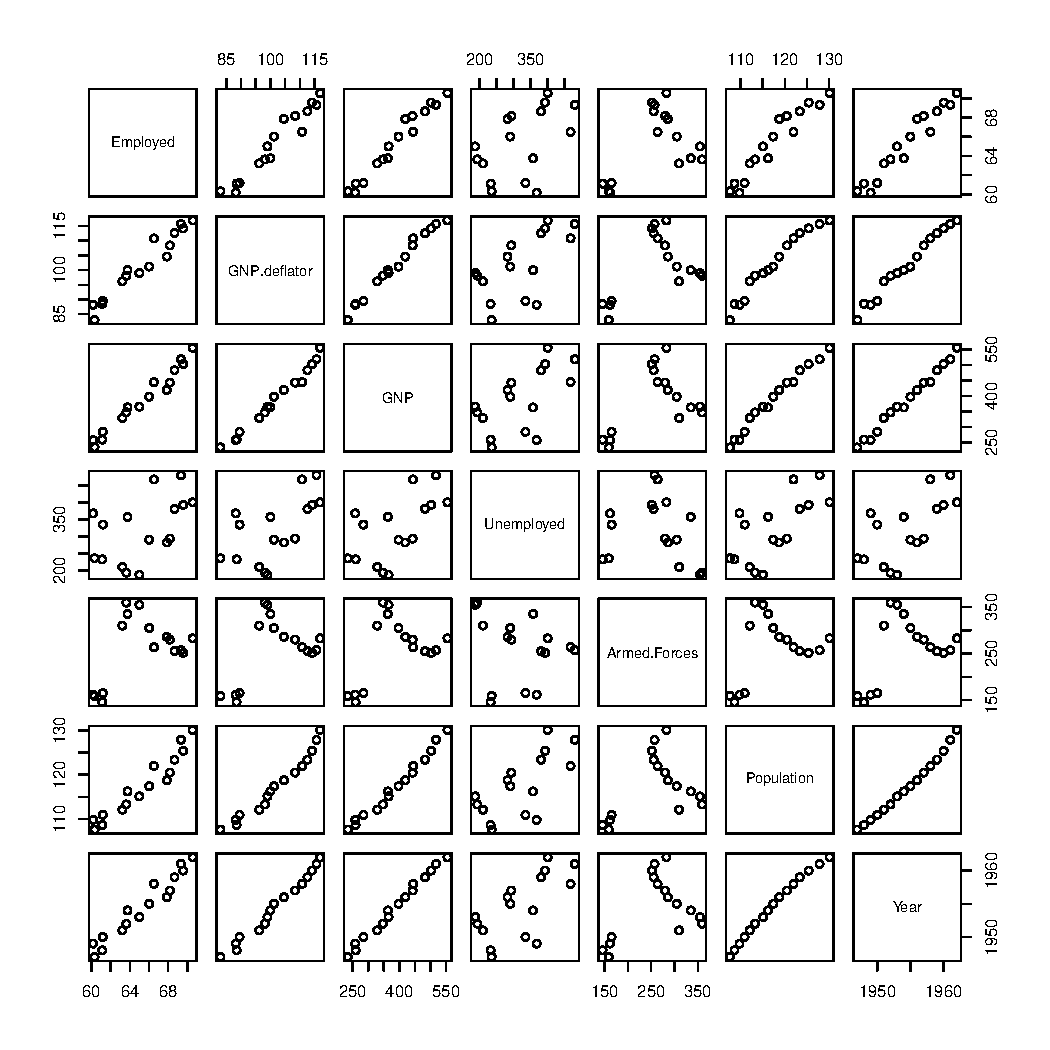
\includegraphics[height=3in]{longley-pairs}}
\end{frame}

\begin{frame}[fragile]
  \frametitle{OLS}
\begin{small}
\begin{verbatim}
> longley.lm = lm(Employed ~ ., data=longley)
> summary(longley.lm)

Coefficients:
               Estimate Std. Error t value Pr(>|t|)
(Intercept)  -3.482e+03  8.904e+02  -3.911 0.003560 **
GNP.deflator  1.506e-02  8.492e-02   0.177 0.863141
GNP          -3.582e-02  3.349e-02  -1.070 0.312681
Unemployed   -2.020e-02  4.884e-03  -4.136 0.002535 **
Armed.Forces -1.033e-02  2.143e-03  -4.822 0.000944 ***
Population   -5.110e-02  2.261e-01  -0.226 0.826212
Year          1.829e+00  4.555e-01   4.016 0.003037 **
---
Signif. codes:  0 '***' 0.001 '**' 0.01 '*' 0.05 '.' 0.1 ' ' 1

Residual standard error: 0.3049 on 9 degrees of freedom
Multiple R-squared: 0.9955,	Adjusted R-squared: 0.9925
F-statistic: 330.3 on 6 and 9 DF,  p-value: 4.984e-10
\end{verbatim}
\end{small}
\end{frame}
\begin{frame}
  \frametitle{Ridge Trace}
  \centerline{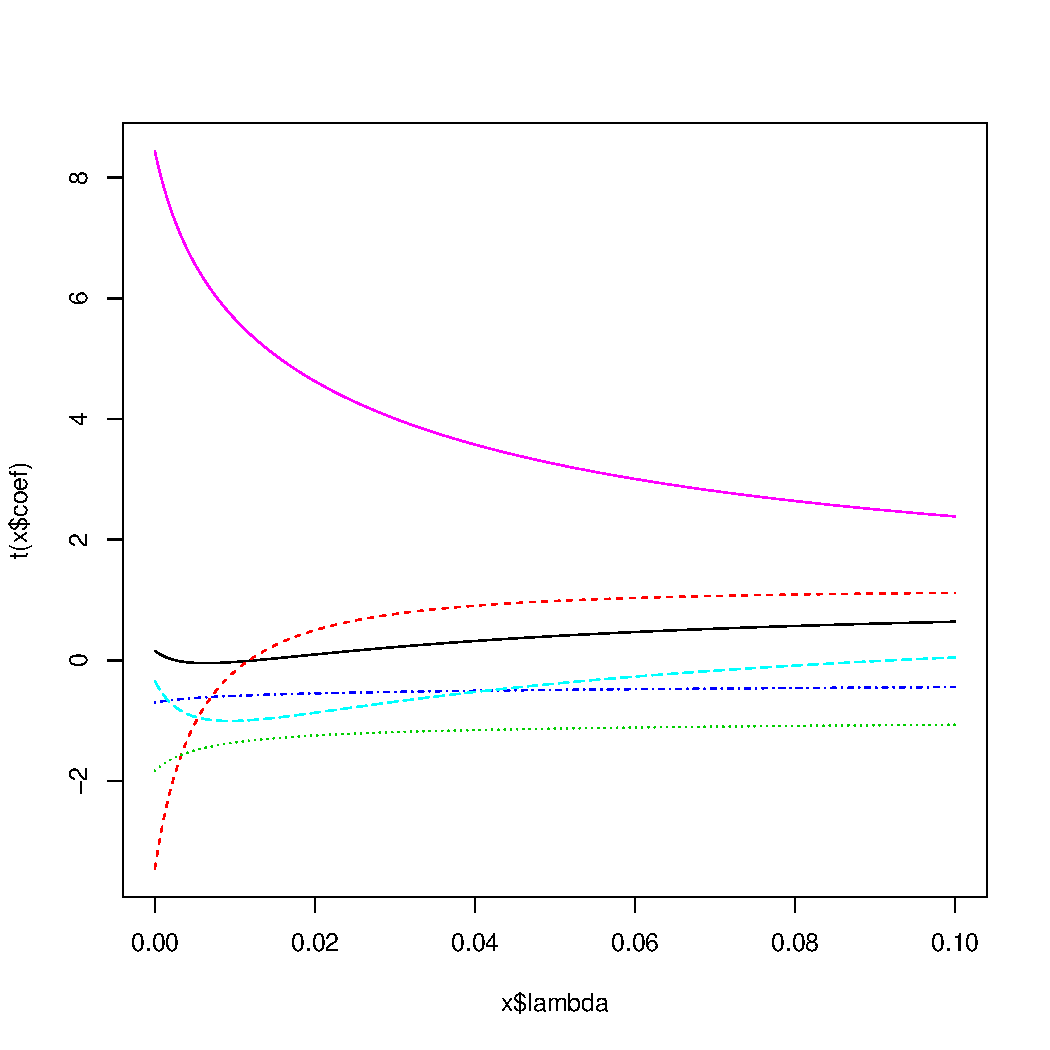
\includegraphics[height=3in]{ridge-trace}}
\end{frame}
\begin{frame}[fragile]
\frametitle{Generalized Cross-validation}
\begin{small}
\begin{verbatim}
> select(lm.ridge(Employed ~ ., data=longley,
         lambda=seq(0, 0.1, 0.0001)))

modified HKB estimator is 0.004275357
modified L-W estimator is 0.03229531
smallest value of GCV  at 0.0028

> longley.RReg = lm.ridge(Employed ~ ., data=longley,
                          lambda=0.0028)
> coef(longley.RReg)
           GNP.deflator    GNP     Unemployed  Armed.Forces
-2.950e+03 -5.381e-04   -1.822e-02  -1.76e-02 -9.607e-03

 Population     Year
-1.185e-01  1.557e+00
\end{verbatim}

\end{small}

\end{frame}

\begin{frame} \frametitle{Testimators}

Goldstein \& Smith (1974) have shown that if

\begin{enumerate}
\item
$0 \leq  h_i \leq 1$ and  $\tilde{\gamma}_i = h_i \hat{\gamma}_i$
\item $\frac{\gamma^2_i}{\Var(\hat{\gamma}_i)} < \frac{1 + h_i}{1 - h_i}$
\end{enumerate}
then   $\tilde{\gamma}_i$ has smaller MSE than $\hat{\gamma}_i$

\vspace{14pt}
Case:  If $\gamma_j < \Var(\hat{\gamma}_i) = \sigma^2/l_i^2$  then
$h_i = 0$ and $\tilde{\gamma}_i$ is better.

\vspace{11pt}
Apply: Estimate $\sigma^2$ with SSE/(n - p - 1) and $\gamma_i$ with
$\hat{\gamma}_i$.  Set $h_i = 0$ if t-statistic is less than 1.
\vfill
``testimator'' - see also Sclove (JASA 1968) and Copas ( JRSSB 1983)
\end{frame}
\begin{frame} \frametitle{Generalized Ridge}


Instead of $\gamma_j \simiid \N(0, \sigma^2/k)$ take

$$\gamma_j \ind \N(0, \sigma^2/k_i)$$  \pause

Then Condition of Goldstein \& Smith becomes

$$
\gamma_i^2 < \sigma^2\left[ \frac{2}{k_j} + \frac{1}{l_i^2}  \right]
$$ \pause
\begin{itemize}
\item
If $l_i$ is small almost any $k_i$ will improve over OLS \pause
\item
if $l_i^2$ is large then only very small values of $k_i$ will give an
improvement \pause
\item Prior on $k_i$?   \pause
\item Induced prior on $\b$?
$$\gamma_j \ind \N(0, \sigma^2/k_i) \Leftrightarrow
\b \sim \N(\zero, \sigma^2 \V K^{-1} \V^T)$$
which is not diagonal.   Loss of invariance.
\end{itemize}

\end{frame}
\begin{frame} \frametitle{Summary }

  \begin{itemize}
  \item OLS can clearly be dominated by other estimators
  \item Lead to Bayes like estimators
  \item choice of penalities or prior hyperparameters
  \item hierarchical model with prior on $k_i$
  \end{itemize}

\end{frame}
\end{document}

